% ====================
\chapter{Identifying a Parking Spot}
% ====================

% • In a paper you MUST provide the details, but FIRST convey the idea
% • Introduce the problem, and your idea, using EXAMPLES and only then
% present the general case
% • Explain it as if you were speaking to someone using a whiteboard
% • Conveying the intuition is primary, not secondary
% • Once your reader has the intuition, she can follow the details (but not vice
% versa)
% Even if she skips the details, she still takes away something valuable
% Evidence
% • Your introduction makes claims; The body of the paper provides evidence to
% support each claim
% • Check each claim in the introduction, identify the evidence, and forward-
% reference it from the claim
% • Evidence can be: analysis and comparison, theorems, measurements, case
% studies

% ====================
\section{General Idea}
% ====================
We first address the problem of identifying a suitable parking spot for a
wheelchair in an indoor environment. The identified parking spot will then be
used as a goal state for a planner to subsequently move the robot to.

We start with the following assumptions, for initial simplicity:
\begin{itemize}
\item The algorithm will work in an indoor environment. Objects on the floor
include but are not limited to: chairs, other wheelchairs, tables and cabinets.
\item The algorithm will not deal with moving objects in the scene
\item The floor will be flat throughout (i.e. no ramps)
\item The suitable parking spot in question is entirely in view of the camera.
In practice this means the parking spot is visible to the RGB-D camera 
the parking spot is not overshadowed by any obstacle.
\end{itemize}



% ====================
\section{Problem formulation}
% ====================

[TODO clean up]
Many methods formulate the problem of identifying a parking spot
as a detection problem, where a parking spot is to be detected within the scene.
We instead 
We formulate the problem as follows: General Bayesian/MDP formulation?

\subsection{Definitions}

\begin{itemize}
\item Configuration space
\item Pointcloud space
\item 2D Map space
\item Ground Map
\item Object Map
\item Unknown Map
\item Feasible states
\item Desirability function
\end{itemize}

\subsection{Characteristics of a good parking spot}
\begin{itemize}
\item Minimize 'useless' space, space that another wheelchair cannot fit in 
\item minimize tight spaces, holes, blockades
\item be parallel/perpendicular to walls
\item must be reachable from the current location in a reasonable amount of
time: one smooth motion instead of many iterations of forward/reversing
\item related: takes into account non-holonomic constraints
\item maximize usable free space, minimize wasted space
\item maximize the amount of contiguous space: space that is wide open is more
desirable
\item ensure wheelchair's 'safety': a margin of error, the parking spot
shouldn't be directly touching any objects
\end{itemize}

We return to these characteristics during evaluation in section [TODO], where we
develop quantatitive measures.


\subsection{Our Approach}
\begin{figure}
\centering
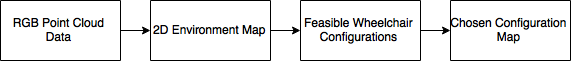
\includegraphics[width=3in]{figures/rgbdmap.png}
\caption{Pipeline for choosing a suitable parking spot.
The transition from point cloud data to a 2D environment map is described in
\autoref{sec:processingPointCloud} and \autoref{sec:2dmap}. Generating feasible configurations from the
environment map is described in \autoref{sec:feasibleparkingspot}. Selecting one
of the feasible configurations is described in
\autoref{sec:choosingparkingspot}.}
\label{fig:rgbdmap}
\end{figure}

\autoref{fig:rgbdmap} shows the general pipeline of the approach taken. The
point cloud data is transformed into a 2D environment map consisting of objects,
ground (free space), and unknown space. From this, the set of feasible
wheelchair configurations are determined, and a heuristic-based desirability
function is applied to choose an appropriate configuration from the feasible set.



% ====================
\section{Data Set}
\label{sec:rgbddataset}
% ====================
A data set of RGBD video is obtained by attaching an Asus Xtion Pro Live onto a
(Wheelchair Model) power wheelchair. Obstacles such as chairs, other
wheelchairs, tables and cabinets are laid out in an indoor office environment to
simulate instances where a wheelchair would potentially park.

[x] different instances are recorded. In each instance, the wheelchair starts
from afar, and is drive into the parking spot, reversed out, then moved
laterally and rotationally. At every point in the video, the position of the
parking spot is within sight of the camera, with the assumption that the back-in
algorithm will only be run if the wheelchair is already pointed in the general
area.

A 3D model of the wheelchair used is also obtained using the Kinect Fusion
algorithm [cite]. This allows for precise simulations of how large the
wheelchair is.

\begin{figure}
\centering
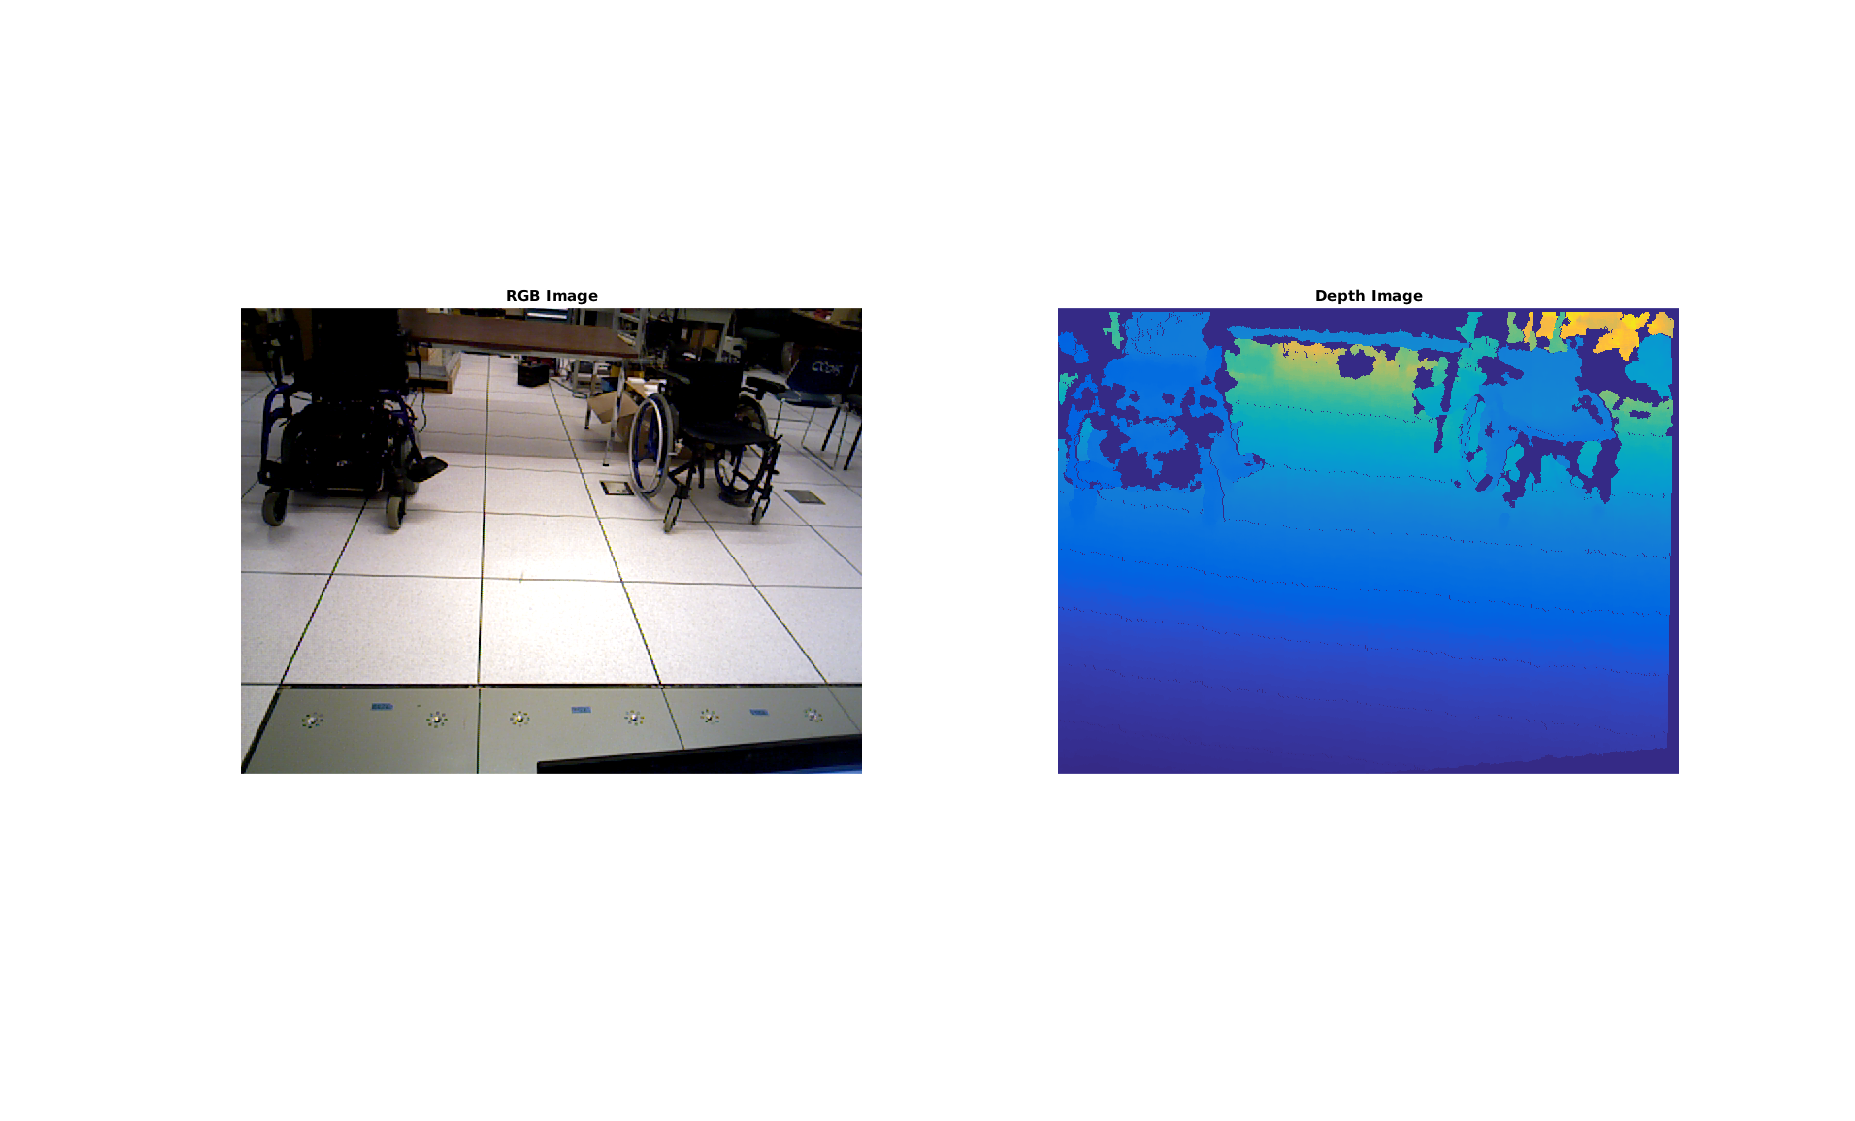
\includegraphics[width=3in]{figures/rgbdwheelchair.png}
\caption{RGB and Depth images as seen by the wheelchair. The objective is to
identify a suitable location within the image for back-in parking.}
\label{fig:rgbdwheelchair}
\end{figure}


% ====================
\section{Preprocessing the Point Cloud}
\label{sec:processingPointCloud}
% ====================
To make a map, we are inspired by the approaches of Holz \cite{holz2013towards}
and Gritti \cite{gritti2014kinect} to detect obstacles based on their height
from the ground plane. This will allow detection of obstacles regardless of
their shape.

One may argue: why not go directly from RGB-D sensor data to classification of
parking spots, instead of a pipeline approach?
First, we will see that ground detection is fairly robust and computationally
cheap: there is very little error in this preprocessing step.
Second, RGB-D data varies quite a bit; there is no clear mapping from RGB-D
point clouds to location of parking spots. A learning approach would require an
overbearing amount of training examples.

First, the point cloud is downsampled using a voxelized grid approach with a 1mm
grid filter. This reduces the computational load and prevents excess weighting of
certain volumes in the upcoming ground plane detection.

Next, parameter estimation must be done to estimate the ground plane. Multiple methods
exist, including RANSAC, Hough transform, and M-estimators
\cite{holz2013towards}.
We use a modified version of RANSAC to estimate the ground plane. The
ground plane is needed for two reasons:
it allows a 2D map to be taken relative to the ground plane, and an obstacle can
be characterized by any point that resides above the ground plane.

Ground plane detection is done on individual frames for robustness to changing
angles of the camera.
Algorithm \autoref{alg:modifiedRansac} shows the modified version of RANSAC,
which results in a ground plane represented as a 4-tuple $(a,b,c,d)$ satisfying
$ax + by + cz + d = 0$. Lines 7-9 highlight the modification with an additional
constraint to avoid detecting vertical planar surfaces (i.e. walls).


\begin{algorithm}
\caption{Modified RANSAC}
\label{alg:modifiedRansac}
\begin{algorithmic}[1]
\Require{
$k$ is the number of iterations to run, P are points in $\mathbb{R}^3$ with the
positive $y$ axis roughly vertical upwards, $\theta_{max}$ is the maximum
inclination angle, $t$ is the threshold used to identify if a point fits the
plane}
\Statex
\Function{ModifiedRANSAC}{$k, P, \theta_{max}, t$}
    \State $n \gets 3$, the minimum number of points to specify a plane
    \State $d \gets 0$, the number of points that lie on the current best plane
    \For{$k$ iterations}
        \State Draw a sample of $n$ non-collinear points from $P$ uniformly at random
        \State $l \gets$ the plane that includes all $n$ points
        \If{the angle between the x-z axis and plane $l$ is greater than $\theta_{max}$}
            \State the plane is too steep, continue to the next iteration
        \EndIf
        \State Find the subset of points $p \in P$ such that all points in $p$ are
        within distance $t$ from plane $l$
        \If{$|p| > d$}
            \State $bestPlane \gets l$, the current best ground plane candidate.
            \State $d \gets |p|$
        \EndIf
    \EndFor
    \State ensure $bestPlane$ has a positive $y$ coefficient ($b$) for consistency
\EndFunction
\Statex
\Ensure{$bestPlane$, a 4-tuple $(a,b,c,d)$ that satisfies $ax + by + cz + d =
0$ representing the ground plane}
\end{algorithmic}
\end{algorithm}

The coordinate system for the point cloud is then rotated so the resulting
ground plane is aligned with the x-y plane. \autoref{fig:pointclouds} shows an
example of the detected ground plane and the rotation to align the ground plane
to the x-y plane.

\begin{figure}
\centering
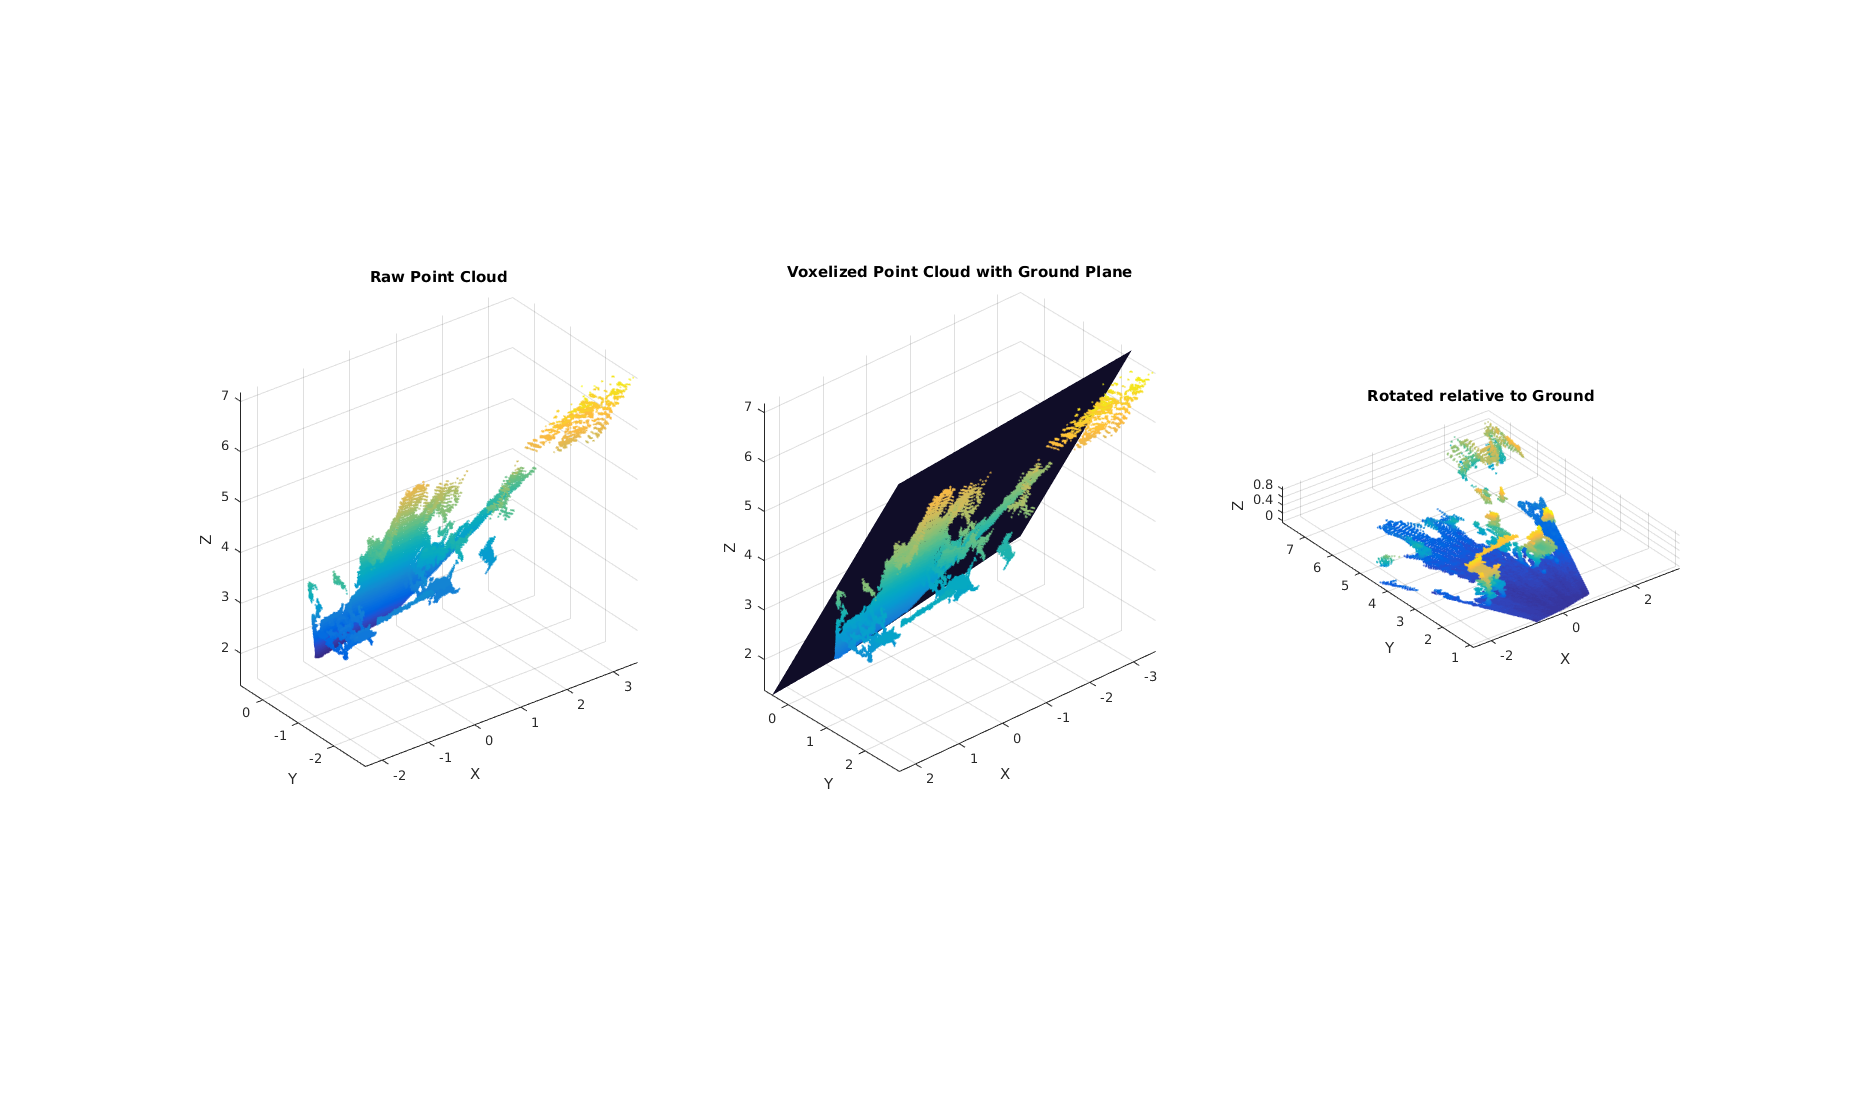
\includegraphics[width=6in]{figures/pointclouds.png}
\caption{Left: point cloud obtained from the RGBD sensor. Middle:
Downsampled point cloud with ground plane detected. Right: Rotated point cloud.}
\label{fig:pointclouds}
\end{figure}

% ====================
\subsection{Rotation Matrix}
% ====================
TODO Rotation matrix equations

% ====================
\subsection{Ground Plane Detection Evaluation}
% ====================
Experiment: 
\begin{itemize}
\item Repeat for 2 videos: flat ground, going on ramps
\item check if first and last frames are correct
\item see change in parameters/angle of ground. Plot
\item state accuracy
\item test for speed
\end{itemize}

% ====================
\section{Generating a 2D Map}
\label{sec:2dmap}
% ====================
The 2D Map is generated by projecting the 3D ground-aligned point cloud onto the
ground plane.
Algorithm \autoref{alg:groundmapprojection} shows how the point cloud is
converted to 2D histograms of object and ground locations. 
A Gaussian blur with
a standard deviation of 0.7 is applied to filter out holes due to noise and
include a safety buffer. This is binarized on lines 12 and 13 by thresholding at
zero, resulting in a binary object map.
Similarly, the 2D ground histogram is binarized on lines 14 and 15 by first applying a Gaussian
blur with a standard deviation of 0.5 and thresholding at zero. 
Additionally, a 1m circle around the origin of the camera is assumed to be
viable positions in the ground map, which accounts for the minimimum range of
the RGBD camera. This is needed to ensure connectivity between the origin state
and farther feasible states, needed on line 2 in algorithm
\autoref{alg:feasibilitycheck}.

TODO talk about morphological dilation and erosion.

In a conservative fashion, any true pixels in the ground map that share a true
value in the object map is set to false, making the set of ground pixels and
object pixels mutually exclusive. 
% A third map is created for pixels that are not classified as a ground or object;
% hence each pixel must be classified as either on the ground plane, an object, or
% unknown.

\begin{algorithm}
\caption{Ground Map Projection}
\label{alg:groundmapprojection}
\begin{algorithmic}[1]
\Require{$P_{rotated}$, $gridStepSize$, $groundThreshold$}
\Statex
\Function{GroundMapProjection}{$P_{rotated}, gridStepSize, groundThreshold$}
    \State $groundMap$, a 2D Histogram with bins spaced $gridStepSize$ metres apart
    \State $objectMap$, a 2D Histogram with bins spaced $gridStepSize$ metres apart
    \For{each point $p \in P_{rotated}$}
        \State $(x,y,z) \gets p$
        \If{$z < groundThreshold$}
            \State add $1$ to the appropriate $groundMap$ bin based on $(x,y)$
        \Else
            \State add $1$ to the appropriate $objectMap$ bin based on $(x,y)$
        \EndIf
    \EndFor
    \State $objectMap \gets GaussianBlur(objectMap, \sigma_1)$
    \State $objectMap \gets 1$ for each non-zero bin, $0$ otherwise

    \State $groundMap \gets GaussianBlur(groundMap, \sigma_2)$
    \State $groundMap \gets 0$ for each bin equal to zero and not already in $objectMap$, $1$ otherwise
\EndFunction
\Statex
\Ensure{$groundMap$, a 2D boolean array with values of $1$ representing the
ground, and $objectMap$}, a 2D boolean array with values of $1$ representing
impassible objects.
\end{algorithmic}
\end{algorithm}

\autoref{fig:groundobjectmap} shows an example of the resulting ground and
object map.

\begin{figure}
\centering
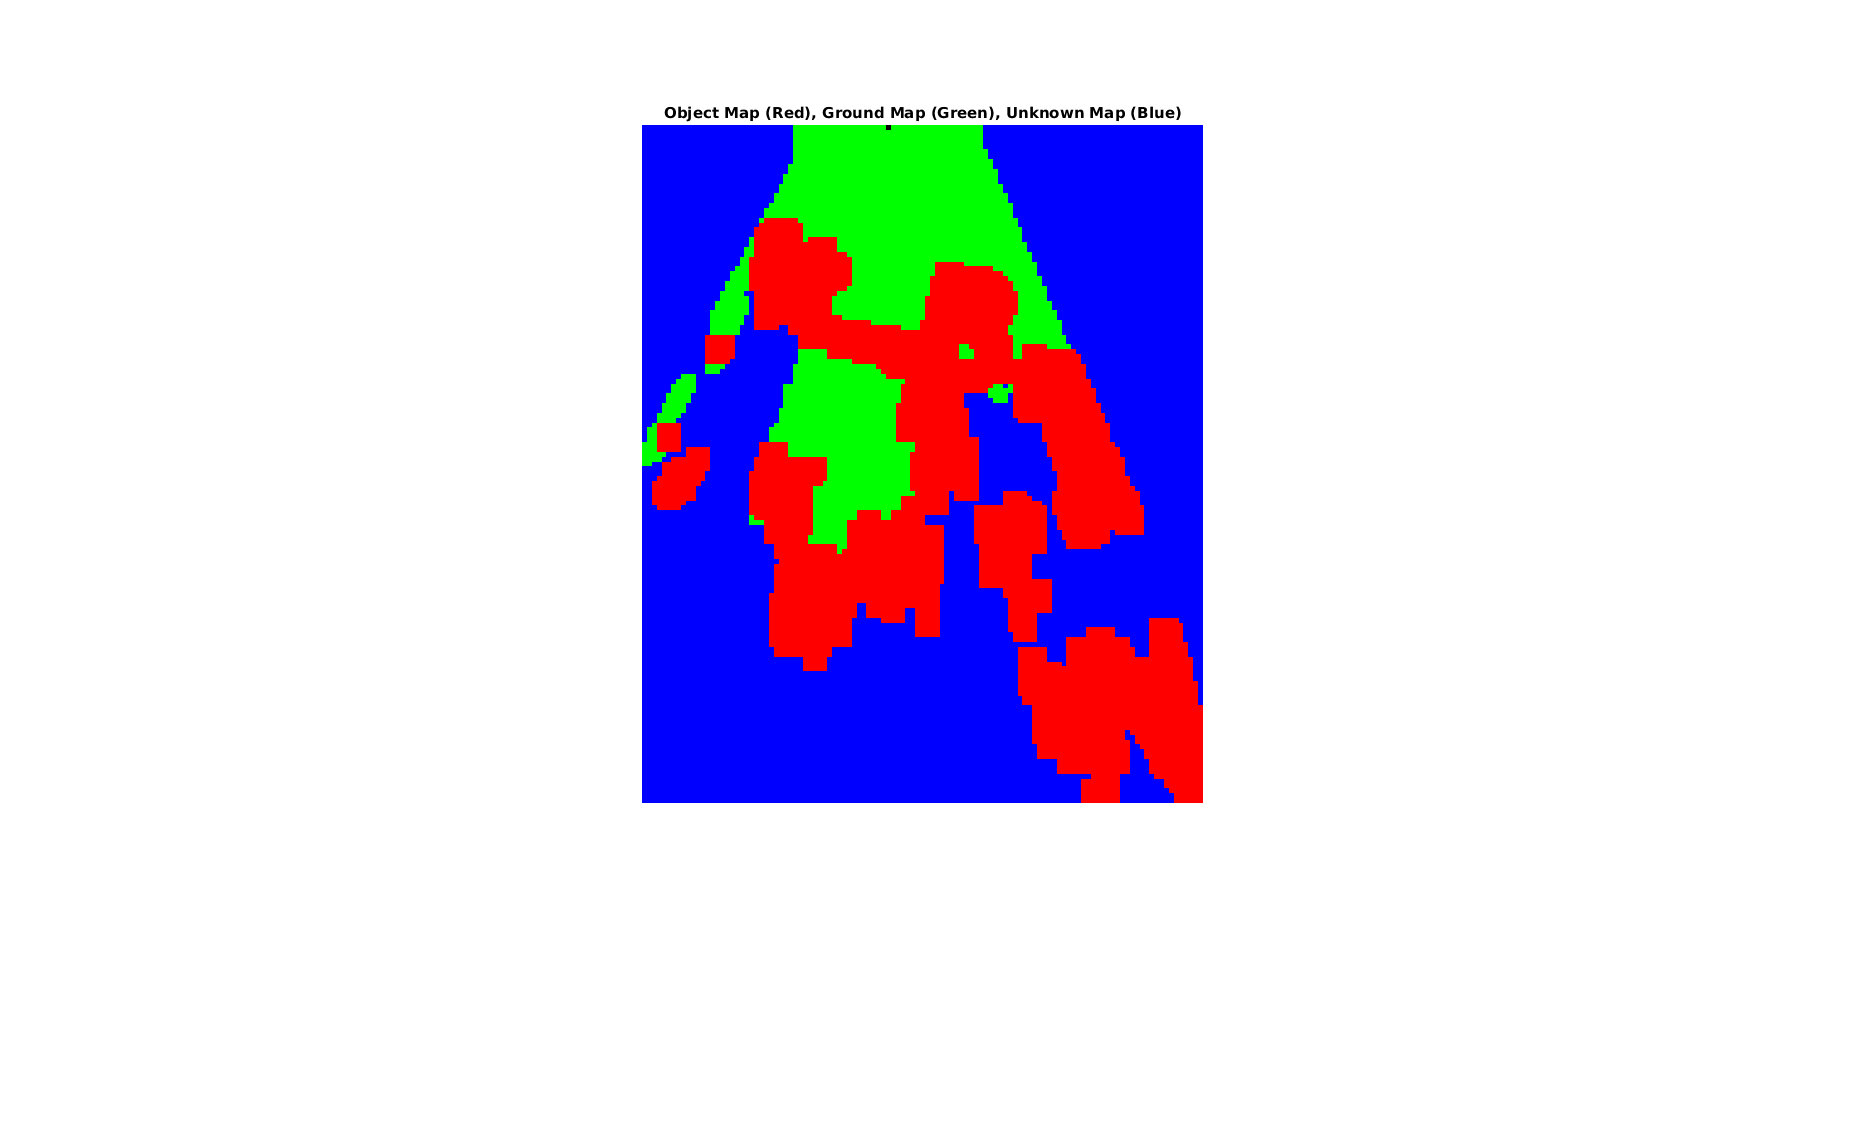
\includegraphics[width=5in]{figures/groundobjectmap.png}
\caption{2D projection of the point cloud. Green (light gray on black and white)
is classified as ground, red (medium gray) is classified as objects, and blue
(dark gray) is classified as unknown, determined by Algorithm
\autoref{alg:groundmapprojection}. The black pixel near the centre top
represents the location of the wheelchair during time of capture.}
\label{fig:groundobjectmap}
\end{figure}

% ====================
\section{Finding Feasible Parking Configurations}
\label{sec:feasibleparkingspot}
% ====================
From a ground map and object map, a set of feasible configurations for the
wheelchair are found. A wheel chair configuration is defined as $(x,y,\theta)$,
where $(x,y)$ define the centre of the wheelchair in the 2D map coordinates of
the ground and object map, and $\theta$ defines a rotation of the wheelchair,
where $\theta = 0$ is the angle of the wheelchair when the point cloud is
captured. Possible values of $\theta$ range from $-10$ to $10$ degrees (TODO
change).

To determine if each configuration for all possible values of $x$, $y$ and
$\theta$ is feasible, three checks are performed, as seen in algorithm
\autoref{alg:feasibilitycheck}. 

The first check is to see if the wheelchair
collides with any objects or is placed on areas not known to be ground. This
performed by checking if each configuration is fully within the ground map area.

The second check is to determine if each configuration can be reached from the
wheelchair's current configuration, the origin $(x_0,y_0,\theta_0)$. $(x_0,y_0)$
is determined from the same transformation used in
\autoref{sec:processingPointCloud} to align the ground plane to the x-y axes.
$\theta_0$ is set to $0$. A flood-fill algorithm is then performed on the
feasible configuration set obtained in the first check to determine all connecting
feasible configurations to the origin $(x_0,y_0,\theta_0)$. Two feasible
configurations are deemed connnected if they are within one manhattan unit of
each other in $x-y-\theta$ space.
Then, feasible configurations from the first check that have no feasible
connecting path to the origin are deemed unreachable and discarded. 
This simplification assumes the possible transitions between states are a one
unit change in $x$, $y$ or $\theta$ (in effect, a holonomic system), instead of
primitive transition curves of a differential drive system
\cite{balkcom2002time}. The ease of computation justifies this choice.


The third check ensures the entirety of the wheelchair falls within the bounds
of the map.

\begin{algorithm}
\caption{Feasibility Check}
\label{alg:feasibilitycheck}
\begin{algorithmic}[1]
\Require{$groundMap, wheelChairMaps, origin$}
\Statex
\Function{FeasibleStates}{$groundMap, wheelChairMaps, origin$}
    \State $feasibleStates \gets$ 1 for all states
    \For{each configuration $c \in$ Configuration Space}
        \State $w \gets wheelChairMaps(c)$
        \State $feasibleStates(c) \gets$ 0 if $w$ is not enclosed in $groundMap$
        \State $feasibleStates(c) \gets$ 0 if $c$ is not connected in configuration space to $origin$
        \State $feasibleStates(c) \gets$ 0 if $w$ collides with edge of map
    \EndFor
\EndFunction
\Statex
\Ensure{$feasibleStates$, a 3D boolean array with values of $1$ representing
feasible configurations of the wheelchair}
\end{algorithmic}
\end{algorithm}

% ====================
\section{Choosing a Suitable Parking Configuration}
\label{sec:choosingparkingspot}
% ====================
% --------------------
\subsection{Formulation}
% --------------------
Given the set of feasible parking spots, we must now choose one of them. What
defines a good parking spot? One could pose this as a supervised learning
problem, given many expert-labeled parking spots on different feasible
configuration sets.  Obtaining meaningful labels, however, is challenging due to
the shear number of possibilities of feasible configuration sets. A
reinforcement learning approach requires defining an appropriate reward
function, which brings us back to the problem of what defines a good parking
spot. We take a heuristics-based approach to develop a potential (reward)
function that is exhaustively evaluated for every configuration.
This obtains a full potential function for the state space, instead of a single
state. The best state may be chosen by taking the state with the maximum
potential.

A good potential function will satisfy the following properties
\begin{itemize}
\item monotonically increasing, allowing for efficient computation
using gradients
\end{itemize}

TODO place in a general framework

We evaluate multiple approaches. We then determine performance based on an
empirical evaluation.

% --------------------
\subsection{Min Convolutions}
% --------------------
From \cite{burcsi2010table}:
Let $x = (x_0, x_1, ..., x_n)$ and $y = (y_0, y_1, ..., y_n)$ be one-dimensional
vectors.
A min-convolution (also known as the (min,+)-convolution) of $x$ and $y$ is the
vector $x \star y = z = (z_0, z_1, ...,z_{2n})$
with $z_m = min(x_i + y_{m-i})$, where the minimum is taken over all possible
values of $i$. 
In contrast, standard convolution, or (+,*)-convolution, is obtained if min is replaced by $\sum$ and
$x_i + y_{m-i}$ by $x_i * y_{m-i}$ , i.e. 
$z_m = \sum(x_i * y_{m-i})$

What I want is (+,min)-convolution, $z_m = \sum min(x_i , y_{m-i})$

I can do this by:
making function A positive, function B negative.
Apply min-convolution.
making function A negative, function B positive.
Apply min-convolution.
do something else.


The only special case we are aware of where a fast algorithm is known for
rank-convolutions is the case when the mask is an axis-parallel box. This case
is common in computer vision and image processing. Rank-convolutions in this
case can be computed in O ( n log n) time; and min- convolution in O ( n) (Gil
and Werman [15]) \cite{babai2009computing}.

Computing min-convolutions when f is arbitrary but g is convex has received
special attention because of its applications to sequence alignment [9] and to
computing distance transforms of images [10]. As pointed out by Eppstein [9],
the problem can be solved in O ( n) time by using the totally monotone matrix
search algorithm of Aggarwal et al. [1].
\cite{babai2009computing}

Felzenszwalb and Huttenlocher [10] developed a different algorithm for the case
when g is convex by noting the relationship between min-convolutions and
lower-envelopes (minimum of a family of functions). The same approach can be
used when g is concave. This algorithm runs in O ( n) time if an intersection
point between shifted copies of g can be computed in constant time. In the worst
case, binary search will find an intersection in O (log n) time, yielding an O (
n log n) algorithm.
\cite{babai2009computing}

% --------------------
\subsection{Algorithm A: Parking lots that maximize usable space}
% --------------------
Algorithm \autoref{alg:generatestatepotentials} shows how a score is given to each
feasible configuration, where higher values correlate to more desirable parking
spots. $w$ in line 3 is a boolean 2D array with values of $1$ representing the
wheelchair at configuration $c$. A squared distance transform is then performed
on the union of $objectMap$ and $w$. This results in $distanceMap$ being the
squared distance of each ground pixel to the closest object to it (with the
wheelchair itself considered an object). This gives a score to each ground pixel:
the farther away the pixel is from all objects, the more desirable the ground
pixel. 

The squared term is included to quadratically favour ground pixels far
away from all objects. This can be reasoned that ground close to objects are less
desirable in a typical wheelchair environment: small areas and cracks between
obstacles are prohibitively small for humans or robots to pass through, and
ground directly next to obstacles risk collision. Ground far from obstacles, on
the other hand, allow for unobstructed movement and ample parking space for
other wheelchairs.

The score for each configuration is then the sum of all the scores for each
ground pixel, as in line 5.

\begin{algorithm}
\caption{Generating State Potentials}
\label{alg:generatestatepotentials}
\begin{algorithmic}[1]
\Require{$groundMap$, $objectMap$}
\Statex
\Function{GenerateStatePotentials}{$objectMap, wheelChairMaps, feasibleStates$}
    \For{each configuration $c \in feasibleStates$}
        \State $w \gets wheelChairMaps(c)$
        \State $distanceMap \gets$ squared distance transform of $objectMap \cup w$
        \State $statePotentials(c) \gets$ sum over all values of $distanceMap$
    \EndFor
\EndFunction
\Statex
\Ensure{$statePotentials$, a configuration-space array where each value
represents the desirability of that configuration.}
\end{algorithmic}
\end{algorithm}

\autoref{fig:desirabilityfunction} shows an example of state potentials
generated from Algorithm \autoref{alg:generatestatepotentials}.

\begin{figure}
\centering
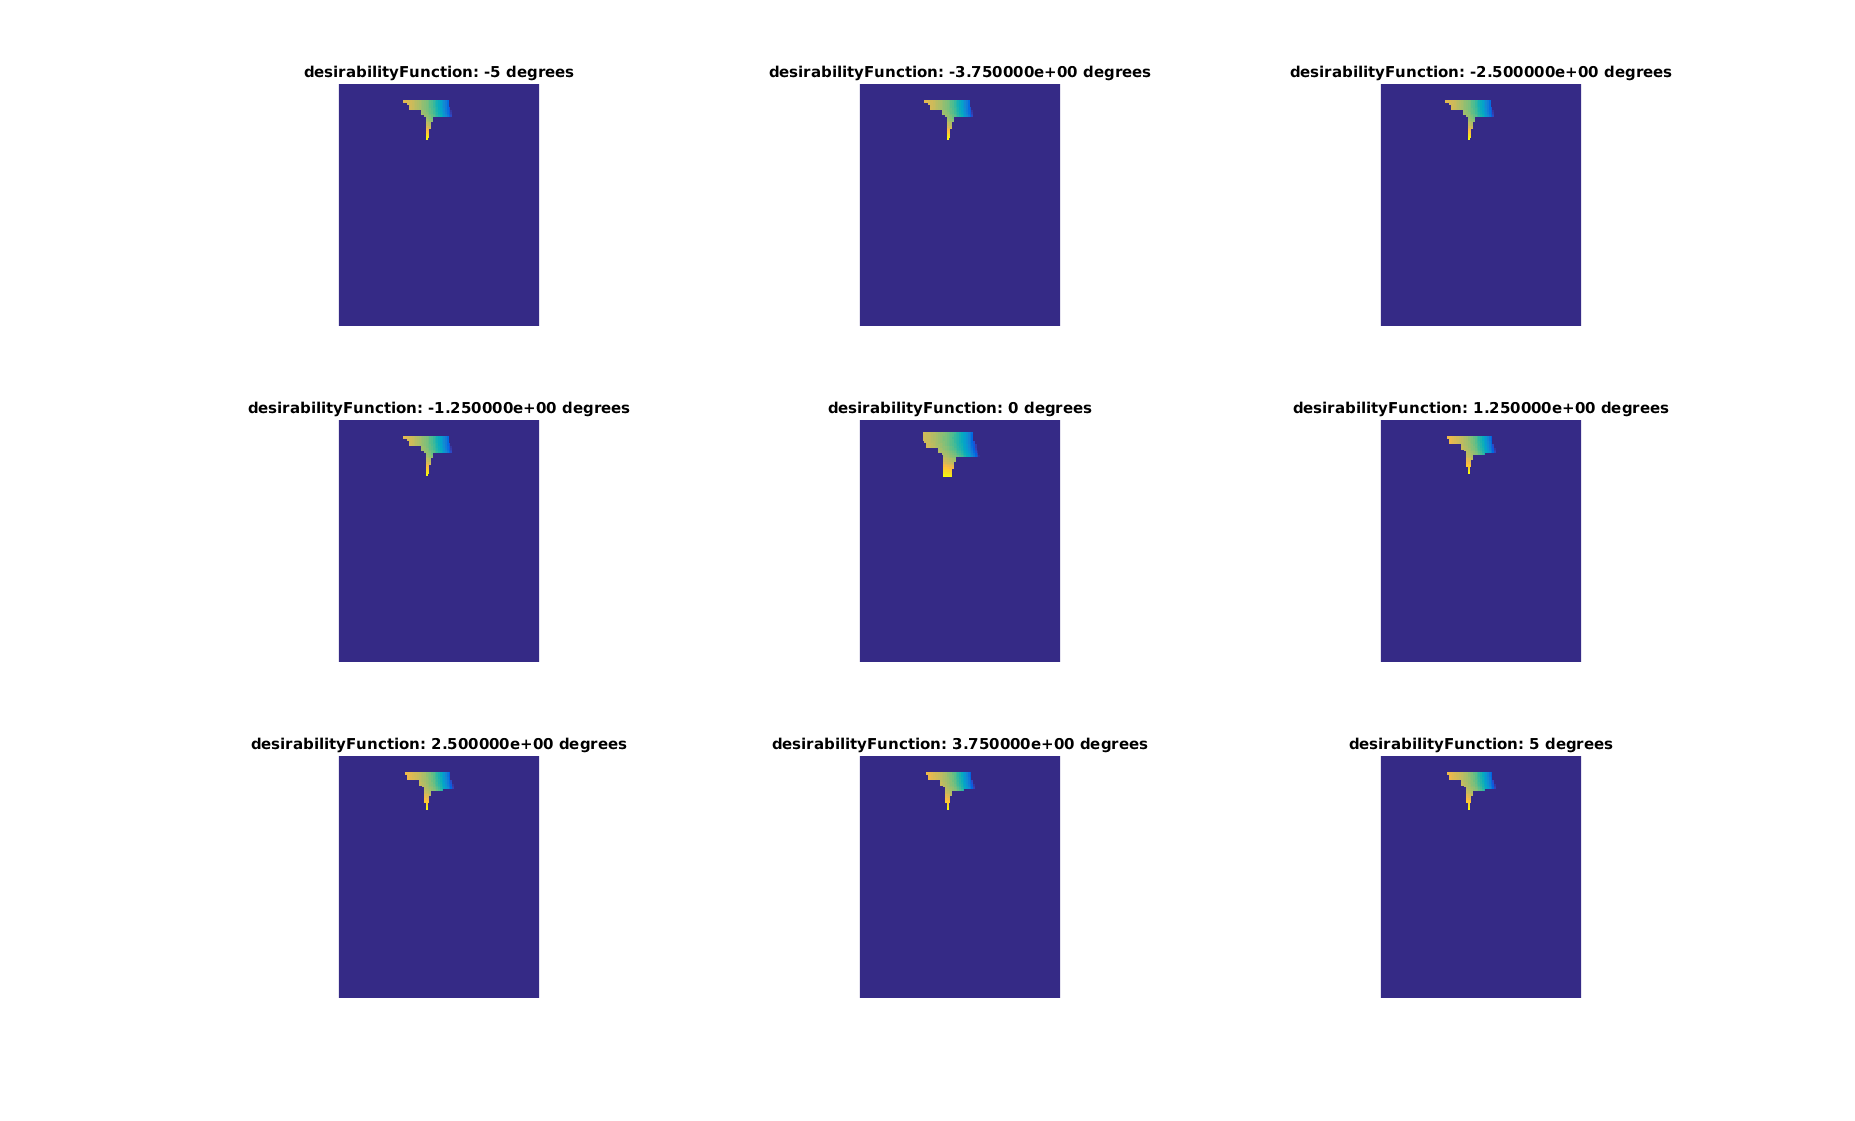
\includegraphics[width=6in]{figures/desirabilityfunction.png}
\caption{Example of a desirability function over a configuration space with 9
different values for $\theta$. Blue (dark) represents low desirability, yellow
(light) represents high desirability. Infeasible configurations determined in 
\autoref{sec:feasibleparkingspot} have desirabilities of $-\infty$.} 
\label{fig:desirabilityfunction}
\end{figure}

% ====================
\section{Efficiency}
% ====================
Efficiency of algorithms.

% ====================
\section{Experiments}
% ====================

\subsection{Simulated Environments}
Toy models: make images in photoshop:
empty room,
room with one object in the centre
room with parking spaces aligned the back
room with two objects in centre, with enough room in-between for a robot

add rotations:
non-axis-aligned parking spots

\subsection{Real-World Environments}

% ====================
\section{Related Work}
\label{sec:parkinglotidentificationlitreview}
% ====================
Detecting a parking spot poses an interesting problem. Unlike a standard object
detection pipeline, a parking spot is not determined by the appearance of an
object, but by the presence of negative space within an area. The context of the
scene also determines where an adequete parking spot should be. In this way, an
ideal parking spot is not purely identifiable by the features within it; but
instead is determined by contextual cues surrounding it.


\subsection{Outdoor Parking Lot Detection}
Work has been done to determine locations of parking spots for cars in car lots
[citations]. 
\cite{wu2006parking, true2007vacant}

Suhr \cite{suhr2010automatic} detects parking spaces in a similar way to ours.
They detect parking spaces by first detecting neighbouring cars using geometric
constraints. Our method, in contrast, does not require such hardcoded
constraints.


Many of these techniques rely on the presence of parking spot
lines, and use line detection algorithms to do so. Once the parking spot is
found, a support vector machine is trained on empty and occupied parking spots.

These methods rely on accurate identification based on line markings, which are
not present in indoor environments not purely dedicated to parking. 

Formulating the problem as a classification problem is then harder, as
classification must be done on any feasible area instead of just a set number of
pre-identified parking spots.

These algorithms also do not address which of the found parking spots to choose:
in a car parking lot, one spot dominates the camera due to the close proximity
of the car to the spots. However, in an indoor wheelchair environment, many
parking lots exists.

TODO researchlog/thesis.org for references.

Many techniques using location-tailored hardware to detect free parking spaces
in car parking lots, involving wireless sensors \cite{panja2011wirelessly},
pre-existing security cameras \cite{true2007vacant} and magnetic field detectors
\cite{boda2007design}. In contrast, our method aims to detect free parking
spaces with only sensors onboard the wheelchair: no external sensors and even no
external pre-determined parking lot spots.


\subsection{Packing Problems}
This problem also has similarities to packing problems. The general packing
problem tries to, given a set of rectangular objects, pack as many as possible
in a larger rectanle. In our case, we are given one wheelchair, and we may wish
to pack it in a space that is least obstrusive to other areas.

TODO researchlog/thesis.org for references.


% *** Packing Problems
% This is a problem in operations research.
% 
% http://en.wikipedia.org/wiki/Packing_problems
% http://www.codeproject.com/Articles/210979/Fast-optimizing-rectangle-packing-algorithm-for-bu
% Problem: In the visible ground, pack as many wheelchairs as possible in it, and then find the best position
% - pack as densely as possible: maximize 'walkable space': space connected to free space
% - constraints: each wheelchair must be able to reach the parking spot
% 
% "Computational Packing Problem"
% http://scholar.google.ca/scholar?q=computational+packing+problem&hl=en&as_sdt=0&as_vis=1&oi=scholart&sa=X&ei=DYxKVeqHHdCNoQT684Eg&ved=0CBsQgQMwAA
% 
% file:papers/hopper2000empirical.pdf
% file:papers/martello2000three.pdf
% 
% Looks like state-of-art:
% http://www.ijcai.org/papers09/Papers/IJCAI09-092.pdf
% 
% I can frame my problem as such:
% - Packing problem, rectangles in arbirtary container
% - with additional constraint of feasability to go from current configuration to target configuration
% 
% *** Tetris Problems
% https://luckytoilet.wordpress.com/2011/05/27/coding-a-tetris-ai-using-a-genetic-algorithm/
% - penalize holes
% - penalize blockades
% 
% **** Tetris is hard, even if the sequence is known
% http://en.wikipedia.org/wiki/Tetris#Computational_complexity


\subsection{Choosing the best parking spot}
\cite{bogoslavskyi2015where} identifies where best to park using an MDP?.

This addresses the issue of how best to choose a parking spot given multiple
candidates. However, it does not work over continuous space, which is what we
have.

\subsection{Choosing the best parking spot, game-theoretic approaches}
Given locations of free car parking spots in a city, Ayala et al.
\cite{ayala2011parking} attempts to choose the ideal parking spot location
in a game-theoretic framework. TODO READ.
\cite{ayala2012parking}

\cite{mejri2014cooperation} uses performance metrics: average distance between
the vehicle and assigned slot, and others.

\cite{alfonsetti2014semi} states: 
As a result, almost all existing methods for parking slot assignment are simple
and greedy approaches, where each car is assigned a free parking slot, which is
closer to its destination. Moreover, no emphasis is placed to optimize the
social benefit of the users during the parking slot assignment. 

\subsection{Path planning with ill-defined goal states}
"Path Planning on Grid Maps with Unknown Goal Poses"

% ====================
\section{Conclusion}
% ====================
